\documentclass{beamer}
\setbeamercovered{transparent}
\usepackage{epstopdf}
\usepackage{listings}
\usepackage{lipsum}
\usepackage{subfig}
\usepackage{algorithm}
\usepackage{algorithmicx}
\usepackage{cite}
\usepackage{lipsum}
\usepackage{amssymb}
\usepackage{color}
\usepackage{IEEEtrantools}
\usepackage{booktabs}
\usepackage{texpower}
\usepackage{amsmath}
\usepackage{caption}
\usepackage{multirow}
\usepackage{graphicx}
\newtheorem{Key points}{Key points}
\newtheorem{Summary}{Summary}
\usepackage{dblfloatfix}
%\usepackage{adjustbox}
%\usepackage{animate}
%\usepackage{movie15}
%\usepackage{subfig}
%\newtheorem{Definition}{Definition}
%\usepackage[font={small}]{caption}
\usepackage{beamerthemeshadow}
\newcommand\Fontvi{\fontsize{5}{6.2}\selectfont}
\newcommand\Fontvia{\fontsize{6}{7.2}\selectfont}
\newcommand\Fontviaa{\fontsize{8}{7.2}\selectfont}
\usepackage{listings}
\lstset{language=C++,
                keywordstyle=\color{blue},
                stringstyle=\color{red},
                commentstyle=\color{magenta},
                morecomment=[l][\color{magenta}]{\#},
                numbers=left,
                escapeinside=||
}

%\captionsetup{font=scriptsize,labelfont=scriptsize}
 \usetheme{Antibes}%PaloAlto
\begin{document}
\title[Lecture 5]{Data Structures} 
\author[]{Ahsan Ijaz}
\date{}
 \frame{\titlepage}
% \AtBeginSection[]
% {
% \begin{frame}<beamer>{Table of Contents}
% \tableofcontents[currentsection,currentsubsection, 
%     hideothersubsections, 
%     sectionstyle=show/shaded,
% ]
% \end{frame}
% }

\section{Containers}
\begin{frame}
  \frametitle{Review}
  \begin{itemize}
  \item<1-> A container class allows you to store an
arbitrary number of things
\item<2-> A sequence container is a container whose
elements can be accessed sequentially.
\item<3-> Sequence containers include vectors,
stacks, queues, lists, and priority queues
(among others).
\item<4-> The performance characteristics of various
sequence containers, and why you might
choose one over another.
  \end{itemize}
\end{frame}
\subsection{Container 1: Stack}
\begin{frame}
  \frametitle{Stack}
  \begin{center}
   \Huge{Let's look at the code STLStack}
  \end{center}
\end{frame}
\subsection{Container 2: Vector}
\begin{frame}
  \frametitle{Vector}
  \begin{center}
    \Huge{Quick Demo: Vector STLVector}
  \end{center}
\end{frame}
\begin{frame}
  \frametitle{STL $<$vector$>$ Push Front}
  Why is there no push\_front method?
  \begin{itemize}
  \item Pushing an element to the front of the vector
requires shifting all other elements in the vector
down by one, which can be very slow.
\item To demonstrate this, let's say we had this nice
little vector:
  \end{itemize}
  \begin{figure}
    \centering
         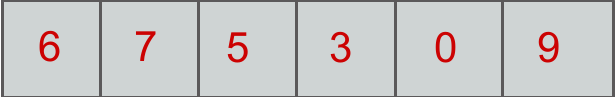
\includegraphics[width=0.7\columnwidth]{vec1.png}
    \caption{Vector}
  \end{figure}

\end{frame}

\begin{frame}
  \frametitle{STL $<$vector$>$ Push Front}
  Now, let's say that push\_front existed, and
 that you wanted to insert an 8 at the beginning
 of this vector.

  \begin{figure}
    \centering
         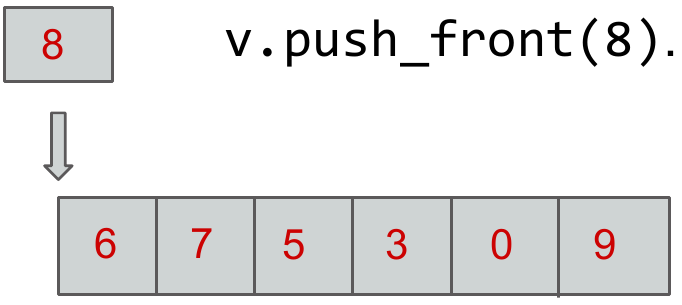
\includegraphics[width=0.7\columnwidth]{vec2.png}
    \caption{Vector}
  \end{figure}

\end{frame}

\begin{frame}
  \frametitle{Push Front}
  First, we may have to expand the capacity of
the vector
\begin{figure}
  \centering
        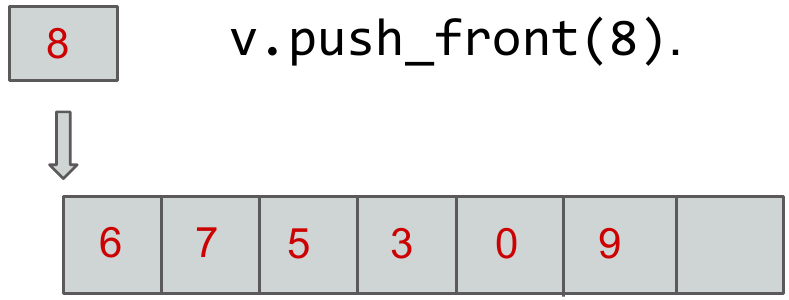
\includegraphics[width=0.7\columnwidth]{vec3.png} 
  \caption{Vector }
\end{figure}
\end{frame}

\begin{frame}
  \frametitle{Push Front}
Then, we'll need to shift every single element
down one position
\begin{figure}
  \centering
        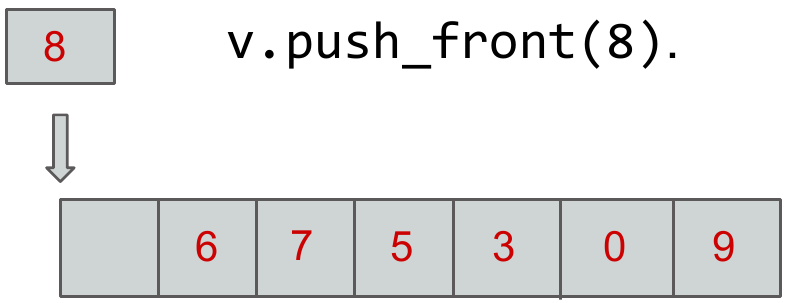
\includegraphics[width=0.7\columnwidth]{vec4.png} 
  \caption{Vector }
\end{figure}
\end{frame}

\begin{frame}
  \frametitle{Push Front}
Finally, we can actually insert the element we
wanted to insert.

\begin{figure}
  \centering
        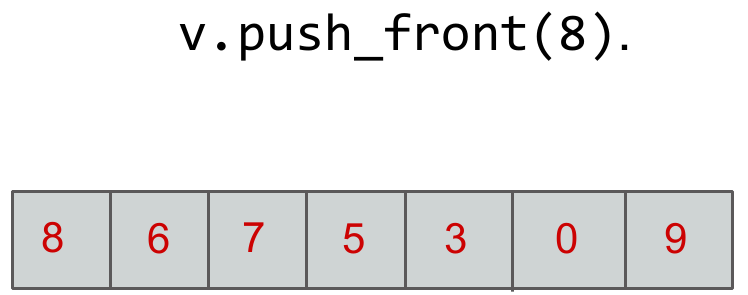
\includegraphics[width=0.7\columnwidth]{vec5.png} 
  \caption{Vector }
\end{figure}
\end{frame}



% \begin{frame}
%    \frametitle{Push front}
%   Now, let's say that push_front existed, and
% that you wanted to insert an 8 at the beginning
% of this vector.
% \begin{figure}
%     \centering
%          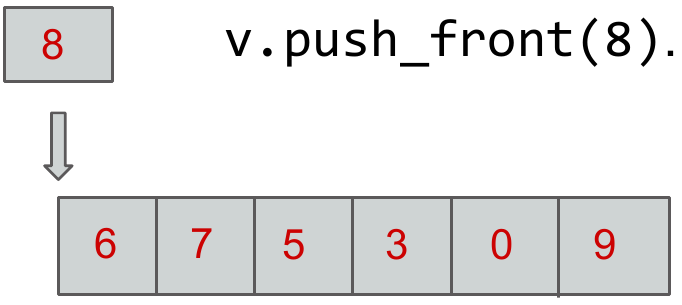
\includegraphics[width=0.7\columnwidth]{vec2.png}
%     \caption{Vector}
%   \end{figure} 
% \end{frame}
\section{Container 3: Deque}
\begin{frame}
  \frametitle{STL $<$deque$>$}
  \begin{itemize}
  \item A deque is a double
ended queue.
\item Unlike a vector, it's possible (and fast) to
push\_front.
\item  The implementation of a deque isn't as
straightforward as a vector though
  \end{itemize}
\end{frame}
\begin{frame}
  \frametitle{Deque}
  \begin{center}
   \Huge{Let's look at the code STLDeque}
  \end{center}
\end{frame}

\begin{frame}
  \frametitle{STL$<$deque$>$: Implementation}
There's no single specification for representing
a deque, but it might be laid out something like
this

\begin{figure}
  \centering
        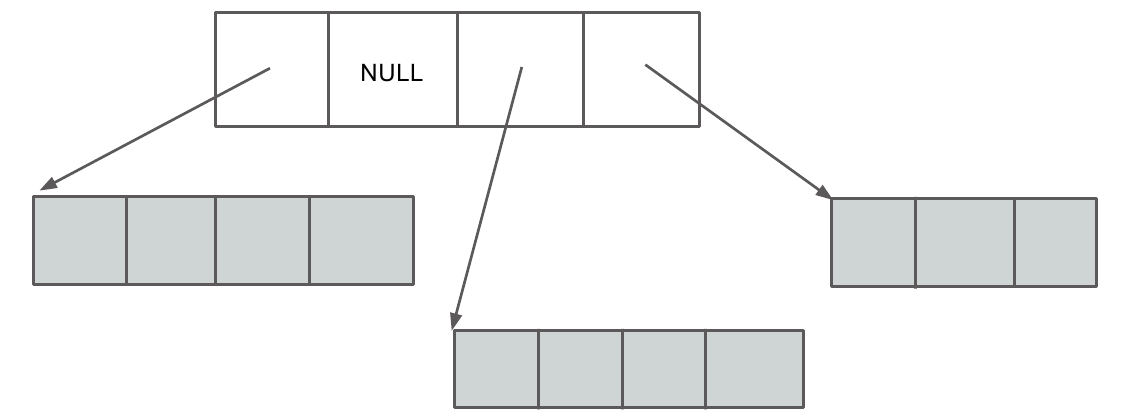
\includegraphics[width=0.7\columnwidth]{deq1.png} 
  \caption{Vector }
\end{figure}
\end{frame}

\begin{frame}
  \frametitle{STL$<$deque$>$: Implementation}
You could support efficient insertion by keeping
some reserved space in front of the vector
representing the first elements of the deque
\begin{figure}
  \centering
        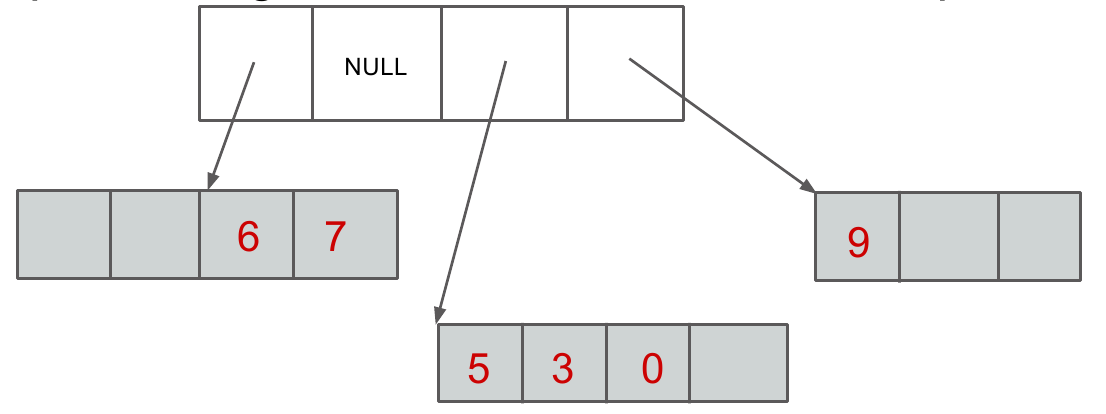
\includegraphics[width=0.7\columnwidth]{deq2.png} 
  \caption{Vector }
\end{figure}
\end{frame}

\begin{frame}
  \frametitle{STL$<$deque$>$: Implementation}
You could support efficient insertion by keeping
some reserved space in front of the vector
representing the first elements of the deque
\begin{figure}
  \centering
        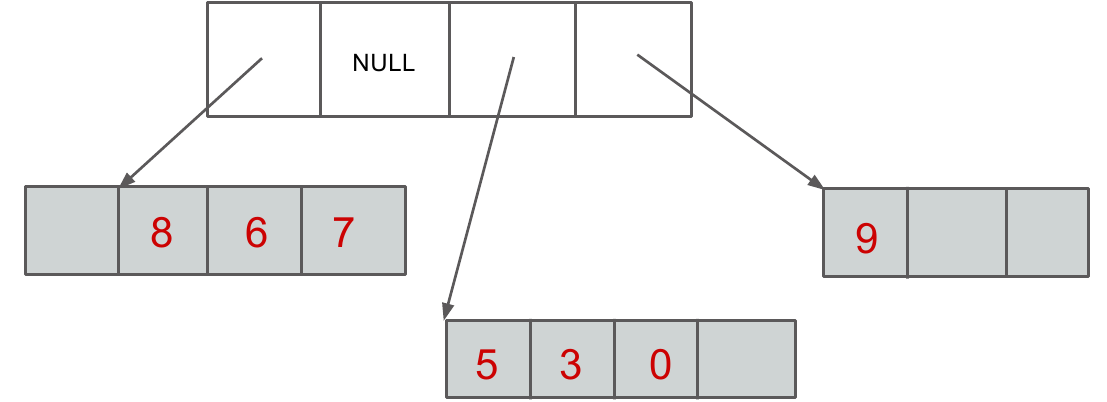
\includegraphics[width=0.7\columnwidth]{deq3.png} 
  \caption{Vector }
\end{figure}
\end{frame}

\begin{frame}
\frametitle{STL $<$deque$>$: Performance}
\begin{itemize}
\item We can now use the push\_front function,
and it will run much faster than if we had
used a vector.
\item However, if all you're doing is iterating,
resizing, and push\_backing, then using a
vector will be faster.
\item Let's see how this looks in real world
performance numbers.
\end{itemize}
\end{frame}

\section{Associative Containers}
\begin{frame}
  \frametitle{Associative Containers}
  \begin{itemize}
  \item Unsurprisingly, associative containers are
containers (objects you can store data in)
\item  Associative containers use the idea of a \textbf{key},
which is used to lookup a value.
\item Maps and Sets are among associative containers.
  \end{itemize}
\end{frame}
\subsection{Container 4: set}
\begin{frame}
  \frametitle{STL$<$set$>$}
  \begin{itemize}
  \item  The set data structure can be thought of as a checklist of items. We can
 add elements to a set, or remove elements from one. Then, we can ask the
 set if it contains a particular item or not.
\item  We can add duplicates, but only one copy will be stored.
 That is because sets are only concerned about whether an item appears in
 the data structure or not.
  \end{itemize}
\end{frame}
\begin{frame}
  \frametitle{STL$<$set$>$}
  \begin{center}
\Huge{ Let's take a quick peek at the code though,
so we can see what STL set code looks like
}    
  \end{center}

\end{frame}

% \subsection{Container 5: Map}
% \begin{frame}
%   \frametitle{STL$<$map$>$}
%   \begin{itemize}
%   \item  The set data structure can be thought of as a checklist of items. We can
%  add elements to a set, or remove elements from one. Then, we can ask the
%  set if it contains a particular item or not.
% \item  We can add duplicates, but only one copy will be stored.
%  That is because sets are only concerned about whether an item appears in
%  the data structure or not.
%   \end{itemize}
% \end{frame}
% \begin{frame}
%   \frametitle{STL$<$map$>$}
%   \begin{center}
% \Huge{ Let's take a quick peek at the code though,
% so we can see what STL set code looks like
% }    
%   \end{center}

% \end{frame}

\section{Iterator}
\begin{frame}
  \frametitle{Iterator: Motivation}
  \begin{itemize}
  \item How do you iterate through all the elements
of a set?
\item  How do you iterate through all the elements
of a map?
  \end{itemize}

Because maps and sets aren't sequence
containers, we can't just go from 0 to vector.
or pop elements off of a stack until it's
empty.
\end{frame}
\begin{frame}
  \frametitle{Iterators: example}
  \begin{center}
    \Large{As we first see them, iterators will allow us to
iterate through all the elements of an
unsequenced collection of elements (like a set
or a map)
}
  \end{center}
\end{frame}
\begin{frame}
  \begin{itemize}
  \item  Let's first try and get a conceptual model of
what an iterator is.
\item Say that we have a set of integers. Say the
set was named 's'.
  \end{itemize}
  \begin{figure}
    \centering
         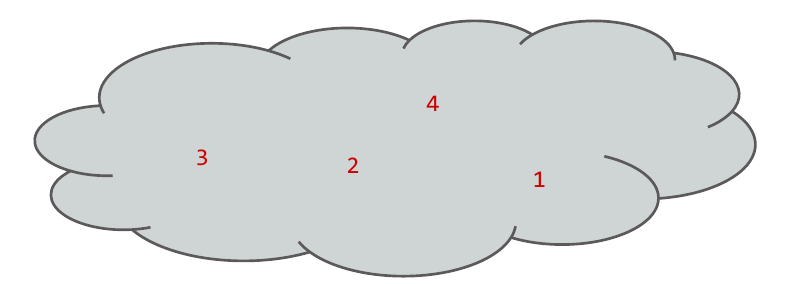
\includegraphics[width=0.9\columnwidth]{itr1.png} 
    \caption{Set Data}
  \end{figure}
\end{frame}

\begin{frame}
  \begin{itemize}
  \item  Let's first try and get a conceptual model of
what an iterator is.
\item Iterators allow us to view an unordered
collection in a linear order
  \end{itemize}
  \begin{figure}
    \centering
         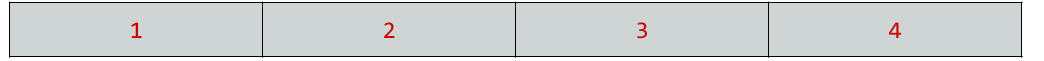
\includegraphics[width=0.9\columnwidth]{itr2.png} 
    \caption{Linear Picture}
  \end{figure}
\end{frame}

\begin{frame}
  \begin{itemize}
  \item  Let's first try and get a conceptual model of
what an iterator is.
\item  We can construct an iterator 'i' to point to the
first element in the set
  \end{itemize}
  \begin{figure}
    \centering
         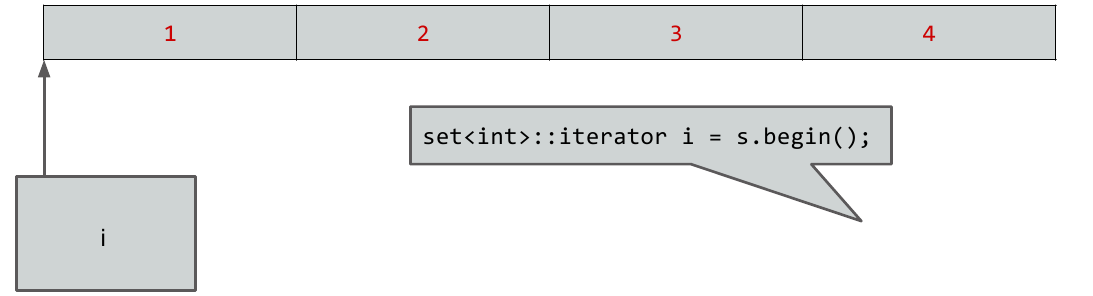
\includegraphics[width=0.9\columnwidth]{itr3.png} 
    \caption{Start a Iterator}
  \end{figure}
\end{frame}
 
\begin{frame}
  \begin{itemize}
  \item  Let's first try and get a conceptual model of
what an iterator is.
\item  We can dereference our iterator to read the
value the iterator is currently on
  \end{itemize}
  \begin{figure}
    \centering
         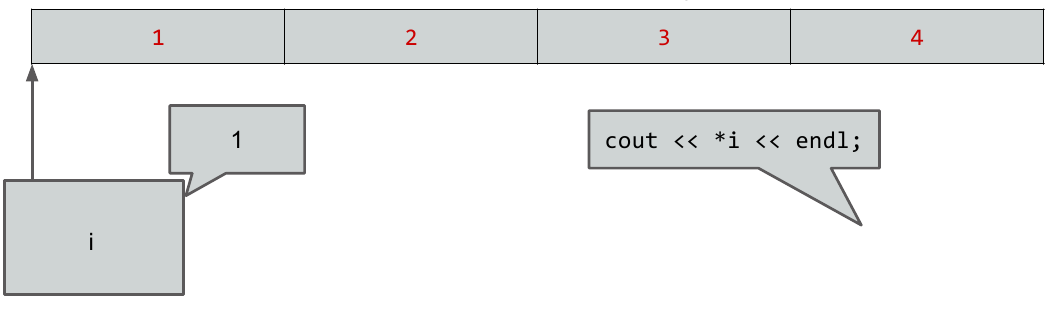
\includegraphics[width=0.9\columnwidth]{itr4.png} 
    \caption{Dereference Iterator}
  \end{figure}
\end{frame}

\begin{frame}
  \begin{itemize}
  \item  Let's first try and get a conceptual model of
what an iterator is.
\item  We can \textbf{advance} our iterator
  \end{itemize}
  \begin{figure}
    \centering
         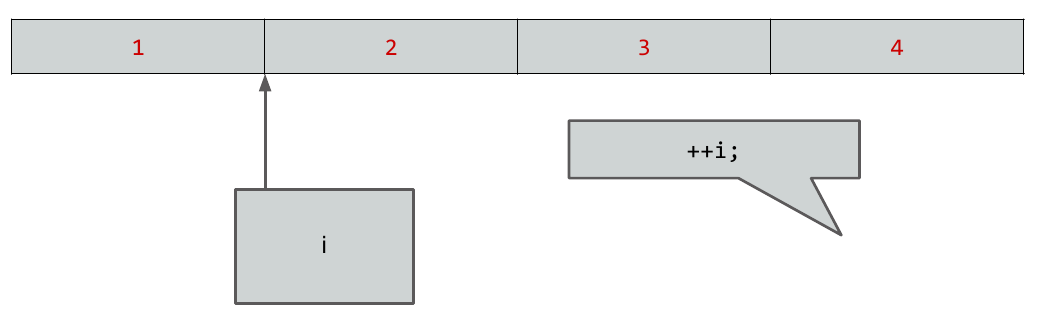
\includegraphics[width=0.9\columnwidth]{itr5.png} 
    \caption{Advancing Iterator}
  \end{figure}
\end{frame}


\begin{frame}
  \begin{itemize}
  \item  Let's first try and get a conceptual model of
what an iterator is.
\item  We can \textbf{dereference} our iterator \textbf{again} and
read a different value
  \end{itemize}
  \begin{figure}
    \centering
         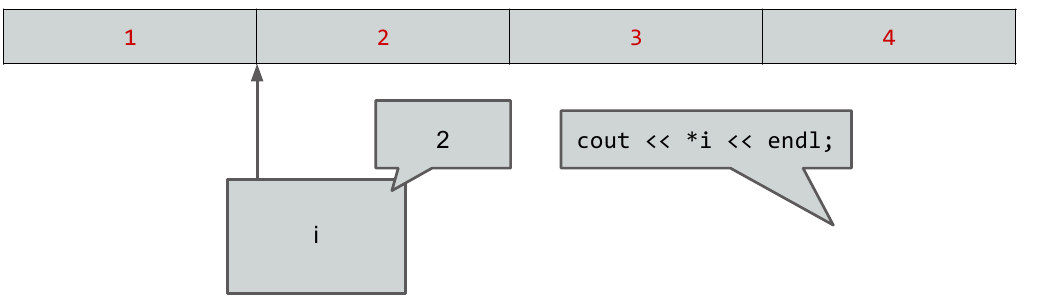
\includegraphics[width=0.9\columnwidth]{itr6.png} 
    \caption{Reading next value}
  \end{figure}
\end{frame}

\begin{frame}[fragile]
  \frametitle{Iterators}
  Eventually, we reach the end of a container.
You can check if an iterator has iterated
through every element in the container by
comparing it to the .end() element.
\begin{lstlisting}
if (i == s.end())
cout << "We're done!" << endl;
\end{lstlisting}
\end{frame}
\begin{frame}
  \frametitle{Iterator}
Remember the four most fundamental iterator
operations:
  \begin{itemize}
  \item 
\item Create an iterator
\item Dereference an iterator and read the value
it's currently looking at
\item Advance an iterator
\item Compare an iterator against another iterator
(especially one from the .end()) method

  \end{itemize}
\end{frame}
\begin{frame}[fragile]
 \frametitle{Other uses of Iterator}
STL containers often use iterators to specify
individual elements inside a container.
\begin{lstlisting}
vector<int> v;
for (int i = 0; i < 10; i++) {
v.push_back(i);
}
v.erase(v.begin() + 5, v.end());
// v now contains 0, 1, 2, 3, 4
\end{lstlisting}
\end{frame}
\begin{frame}
  \frametitle{Other uses of Iterators}
  \begin{itemize}
  \item Iterator's don't always have to iterate through
all of a container.
\item For example, they could iterate through a range
of elements.
  \end{itemize}
\end{frame}
\begin{frame}[fragile]
  \frametitle{Other uses of Iterators}
For example, here's the code to iterate through
all the integers in a set:
\begin{lstlisting}
set<int>::iterator i = s.begin();
set<int>::iterator end = s.end();
while (i != end) {
cout << *i << endl;
++i;
}
\end{lstlisting}
\end{frame}

\begin{frame}[fragile]
  \frametitle{Other uses of Iterators}
For example, here's the code to iterate through
all the integers greater than 7 and less than
23 in a set:
\begin{lstlisting}
set<int>::iterator i = s.lower_bound(7);
set<int>::iterator end = s.upper_bound(23);
while (i != end) {
cout << *i << endl;
++i;
}

\end{lstlisting}
\end{frame}
\end{document}